%%%%%%%%%%%%%%%%%%%%%%%%%%%%%%%%%%%%%%%%%
% a0poster Landscape Poster
% LaTeX Template
% Version 1.0 (22/06/13)
%
% The a0poster class was created by:
% Gerlinde Kettl and Matthias Weiser (tex@kettl.de)
%
% This template has been downloaded from:
% http://www.LaTeXTemplates.com
%
% License:
% CC BY-NC-SA 3.0 (http://creativecommons.org/licenses/by-nc-sa/3.0/)
%
%%%%%%%%%%%%%%%%%%%%%%%%%%%%%%%%%%%%%%%%%

%----------------------------------------------------------------------------------------
%	PACKAGES AND OTHER DOCUMENT CONFIGURATIONS
%----------------------------------------------------------------------------------------

\documentclass[a0,landscape]{a0poster}

\usepackage{multicol} % This is so we can have multiple columns of text side-by-side
\columnsep=100pt % This is the amount of white space between the columns in the poster
\columnseprule=3pt % This is the thickness of the black line between the columns in the poster

\usepackage[svgnames]{xcolor} % Specify colors by their 'svgnames', for a full list of all colors available see here: http://www.latextemplates.com/svgnames-colors

\usepackage{times} % Use the times font
%\usepackage{palatino} % Uncomment to use the Palatino font

\usepackage{graphicx} % Required for including images
\graphicspath{{figures/}} % Location of the graphics files
\usepackage{booktabs} % Top and bottom rules for table
\usepackage[font=small,labelfont=bf]{caption} % Required for specifying captions to tables and figures
\usepackage{amsfonts, amsmath, amsthm, amssymb} % For math fonts, symbols and environments
\usepackage{wrapfig} % Allows wrapping text around tables and figures
\usepackage[utf8]{inputenc} % Pour utiliser les caractères accentués

\begin{document}

%----------------------------------------------------------------------------------------
%	POSTER HEADER
%----------------------------------------------------------------------------------------

% The header is divided into three boxes:
% The first is 55% wide and houses the title, subtitle, names and university/organization
% The second is 25% wide and houses contact information
% The third is 19% wide and houses a logo for your university/organization or a photo of you
% The widths of these boxes can be easily edited to accommodate your content as you see fit

\noindent\begin{minipage}[t]{\linewidth}
\centering
\noindent \veryHuge \color{NavyBlue} \textbf{Lake-river and lake-atmosphere interactions in a changing climate over Northeast Canada} \color{Black}\\ % Title
\vspace{0.5cm}
\noindent\begin{minipage}[b]{0.2\linewidth}
      \center
      
\includegraphics[width=15cm]{logo_cnrcwp_escer.png} % Logo or a photo of you, adjust its dimensions here
\end{minipage}
%
\begin{minipage}[t]{0.6\linewidth} % Author(s)
  \center
  \begin{minipage}[t]{0.4\linewidth}
  \center
  \huge \textbf{Oleksandr Huziy} \\
        \texttt{guziy.sasha@gmail.com}
  \end{minipage}
  %
  \begin{minipage}[t]{0.05\linewidth}
   \center
   \&
  \end{minipage}
  %
  \begin{minipage}[t]{0.4\linewidth}
     \center
     \huge \textbf{Laxmi Sushama} \\
     \texttt{laxmi.sushama@uqam.ca}
  \end{minipage}
\end{minipage}
%
\begin{minipage}[b]{0.18\linewidth}
  \center
  
\includegraphics[width=7cm]{logo_uqam.png} % Logo or a photo of you, adjust its dimensions here
\end{minipage}
\rule{\linewidth}{2pt}
\end{minipage}
%

\vspace{1cm} % A bit of extra whitespace between the header and poster content

%----------------------------------------------------------------------------------------

\begin{multicols}{3} % This is how many columns your poster will be broken into, a poster with many figures may benefit from less columns whereas a text-heavy poster benefits from more

%----------------------------------------------------------------------------------------
%	ABSTRACT
%----------------------------------------------------------------------------------------

\color{Navy} % Navy color for the abstract

\begin{abstract}
Lakes influence the regional climate and hydrology in a number of ways and therefore they should be represented
in climate models in a realistic manner. Lack of representation of lakes in models can lead to errors in simulated
energy and water fluxes, for lake-rich regions. This study focuses on the assessment of the impact of climate
change on lakes and hydrology as well as on the influence of lakes on projected changes to regional climate
and surface hydrology, particularly streamflows, for Northeast Canada. To this end, transient climate change
simulations spanning the 1950–2100 period are performed, with and without lakes, with the fifth generation of
the Canadian Regional Climate Model (CRCM5), driven by the Canadian Earth System Model (CanESM2) at the
lateral boundaries for Representative Concentration Pathway 8.5.

Comparison of projected changes from the CRCM5 simulations with and without lakes suggest that lakes
attenuate projected increases to 2-m air temperature in all seasons, almost everywhere in the study domain, with
maximum decreases of the order of 2$^\circ$C occurring during winter. As for streamflows, results suggest projected
increases for winter and spring and decreases during summer. Comparison of the projected changes suggests
that lakes attenuate the projected increases in streamflows in spring due to the storage effect of lakes, and
also attenuate the projected decreases in streamflows in summer in future climate due to the gradual release of
the excess water stored in the lakes during spring. This study, thus demonstrates the impact of lakes on projected
changes to the regional climate and hydrology for the study region using a single regional modelling system.
\end{abstract}

%----------------------------------------------------------------------------------------
%	INTRODUCTION
%----------------------------------------------------------------------------------------

\color{SaddleBrown} % SaddleBrown color for the introduction

\section*{Introduction}
Inland water bodies, such as lakes and rivers, are essential for human
livelihood (i.e. drinking water, agriculture, hydroelectricity, transportation),
and this has led to many activities around lakes and rivers, which in turn
resulted in the development of expensive and important infrastructure in the
proximity of such water bodies. The safety and proper functioning of these
infrastructures in the context of a changing climate is a major concern. For
this reason, it is important to assess projected changes to the hydrological
cycle and related uncertainties.

Though many climate models, particularly RCMs, include lakes, only few studies
have attempted to realistically simulate the water balance of lakes, considering
inflows and outflows of lakes, and the impact of lakes on streamflows. Huziy and
Sushama (2015) recently implemented a river/lake routing scheme, interflow
process, i.e. the lateral flow of water in the top soil layers along topographic
slopes, and interactions between lakes and rivers in terms of water balance in
the fifth generation Canadian Regional Climate Model (CRCM5). By including lake
routing, they noticed significant improvements to the simulated spring peak and
winter low flows, which were too high and too low, respectively, without the
lake-river interaction. The impacts of interflow on simulated streamflow and on
the regional climate were modest according to their study. These new
implementations in CRCM5 by Huziy and Sushama (2015) resulted in a more
comprehensive tool for regional climate change studies that can be used to
better understand interactions between atmosphere, lakes and rivers in the
context of a changing climate.

This study therefore focuses on the projected changes to the regional climate
and hydrology for northeastern Canada (Fig. 1) using CRCM5, and estimates the
impacts of lake-river, lake-atmosphere interactions and of interflow on the
projected changes to selected hydrologic/near-surface climate variables under
the Representative Concentration Pathway 8.5 (RCP85). For this scenario, the
concentration of greenhouse gases in the atmosphere continues to rise during the
21st century, causing an increase in the radiative forcing of 8.5 ${\rm W/m^2}$ by 2100
with respect to the preindustrial period. The study domain (Fig. 1) covers 21
watersheds that are important for various economic activities (notably
hydropower generation) and contain a large number of subgrid lakes for which the
use of a 1D column lake model is appropriate. The zonal distribution of lakes in
the region is shown in the right panel of Fig. 1. It can be noted that mean lake
fractions reach up to 20\% in the southern and up to 15\% in the northern
basins.

\vspace{1cm}
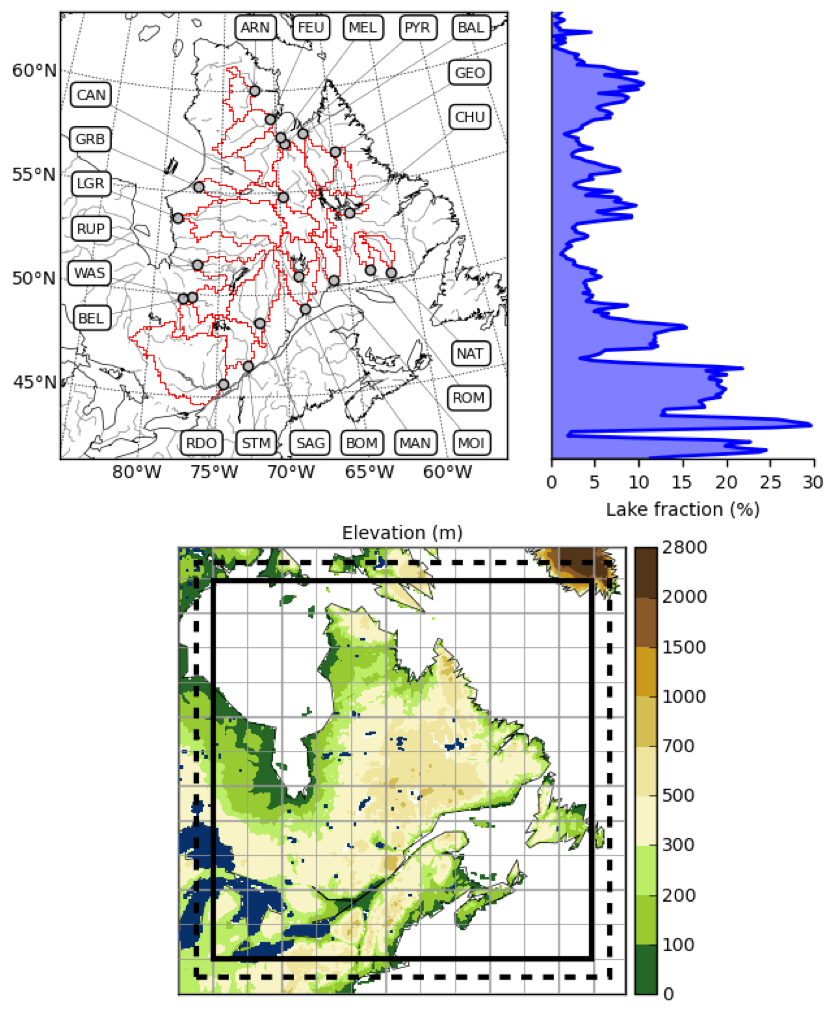
\includegraphics[width=0.4\linewidth]{domain}
\captionof{figure}{\color{Green} The free zone of the simulation domain with
basins of interest (top left panel) and zonally averaged lake fractions (top
right panel); the grey circles show basin outlets determined from the flow
direction field, used for streamflow simulation. Basin boundaries are shown in
red. In the bottom panel, the topography is shown, the cells with lake fractions greater or equal
to 0.6 are indicated with blue colour. The black solid line shows the border
between the free and blending zones. The black dashed line shows the border
between the blending and halo zones. The grey mesh consists of squares
containing 20 by 20 grid cells along each of its edges.}
\vspace{1cm}

%----------------------------------------------------------------------------------------
%	OBJECTIVES
%----------------------------------------------------------------------------------------

\color{DarkSlateGray} % DarkSlateGray color for the rest of the content

\section*{Main Objectives}

\begin{enumerate}
\item Improve most important processes essential for simulating streamflow (rivers, river-lake connectivity, interflow).
\item Study/quantify atm.-lake-river interactions through carefully designed experiments.
\item Study/quantify impact of lake-atmosphere, of lake-river interactions on the projected changes to selected hydrological/near-surface climate variables over northeastern Canada.
\end{enumerate}

%----------------------------------------------------------------------------------------
%	MATERIALS AND METHODS
%----------------------------------------------------------------------------------------

\section*{Materials and Methods}

Fusce magna risus, molestie ut porttitor in, consectetur sed mi. Vestibulum ante ipsum primis in faucibus orci luctus et ultrices posuere cubilia Curae; Pellentesque consectetur blandit pellentesque. Sed odio justo, viverra nec porttitor vel, lacinia a nunc. Suspendisse pulvinar euismod arcu, sit amet accumsan enim fermentum quis. In id mauris ut dui feugiat egestas. Vestibulum ac turpis lacinia nisl commodo sagittis eget sit amet sapien. Phasellus imperdiet, tortor vitae congue bibendum, felis enim sagittis lorem, et volutpat ante orci sagittis mi. Morbi rutrum laoreet semper. Morbi accumsan enim nec tortor consectetur non commodo nisi sollicitudin. Proin sollicitudin. Pellentesque eget orci eros. Fusce ultricies, tellus et pellentesque fringilla, ante massa luctus libero, quis tristique purus urna nec nibh. Proin sollicitudin. Pellentesque eget orci eros. Fusce ultricies, tellus et pellentesque fringilla, ante massa luctus libero, quis tristique purus urna nec nibh.

%------------------------------------------------

\subsection*{Mathematical Section}

Nulla vel nisl sed mauris auctor mollis non sed.

\begin{equation}
E = mc^{2}
\label{eqn:Einstein}
\end{equation}

Curabitur mi sem, pulvinar quis aliquam rutrum. (1) edf (2)
, $\Omega=[-1,1]^3$, maecenas leo est, ornare at. $z=-1$ edf $z=1$ sed interdum felis dapibus sem. $x$ set $y$ ytruem.
Turpis $j$ amet accumsan enim $y$-lacina;
ref $k$-viverra nec porttitor $x$-lacina.

Vestibulum ac diam a odio tempus congue. Vivamus id enim nisi:

\begin{eqnarray}
\cos\bar{\phi}_k Q_{j,k+1,t} + Q_{j,k+1,x}+\frac{\sin^2\bar{\phi}_k}{T\cos\bar{\phi}_k} Q_{j,k+1} &=&\nonumber\\
-\cos\phi_k Q_{j,k,t} + Q_{j,k,x}-\frac{\sin^2\phi_k}{T\cos\phi_k} Q_{j,k}\label{edgek}
\end{eqnarray}
and
\begin{eqnarray}
\cos\bar{\phi}_j Q_{j+1,k,t} + Q_{j+1,k,y}+\frac{\sin^2\bar{\phi}_j}{T\cos\bar{\phi}_j} Q_{j+1,k}&=&\nonumber \\
-\cos\phi_j Q_{j,k,t} + Q_{j,k,y}-\frac{\sin^2\phi_j}{T\cos\phi_j} Q_{j,k}.\label{edgej}
\end{eqnarray}

Nulla sed arcu arcu. Duis et ante gravida orci venenatis tincidunt. Fusce vitae lacinia metus. Pellentesque habitant morbi. $\mathbf{A}\underline{\xi}=\underline{\beta}$ Vim $\underline{\xi}$ enum nidi $3(P+2)^{2}$ lacina. Id feugain $\mathbf{A}$ nun quis; magno. Fusce convallis rutrum turpis, quis aliquet enim accumsan id. Vestibulum ullamcorper porttitor convallis. Integer sagittis interdum malesuada. Class aptent taciti sociosqu ad litora torquent per conubia nostra, per inceptos himenaeos. Sed adipiscing tristique orci at ullamcorper. Morbi accumsan, urna et porttitor pulvinar, lacus risus dignissim massa. Proin sollicitudin. Pellentesque eget orci eros. Fusce ultricies, tellus et pellentesque fringilla, ante massa luctus libero, quis tristique purus urna nec nibh.

%----------------------------------------------------------------------------------------
%	RESULTS
%----------------------------------------------------------------------------------------

\section*{Results}

Donec faucibus purus at tortor egestas eu fermentum dolor facilisis. Maecenas tempor dui eu neque fringilla rutrum. Mauris \emph{lobortis} nisl accumsan. Aenean vitae risus ante. Pellentesque condimentum dui. Etiam sagittis purus non tellus tempor volutpat. Donec et dui non massa tristique adipiscing.
%
\begin{wraptable}{l}{12cm} % Left or right alignment is specified in the first bracket, the width of the table is in the second
\begin{tabular}{l l l}
\toprule
\textbf{Treatments} & \textbf{Response 1} & \textbf{Response 2}\\
\midrule
Treatment 1 & 0.0003262 & 0.562 \\
Treatment 2 & 0.0015681 & 0.910 \\
Treatment 3 & 0.0009271 & 0.296 \\
\bottomrule
\end{tabular}
\captionof{table}{\color{Green} Table caption}
\end{wraptable}
%
Phasellus imperdiet, tortor vitae congue bibendum, felis enim sagittis lorem, et volutpat ante orci sagittis mi. Morbi rutrum laoreet semper. Morbi accumsan enim nec tortor consectetur non commodo nisi sollicitudin. Proin sollicitudin. Pellentesque eget orci eros. Fusce ultricies, tellus et pellentesque fringilla, ante massa luctus libero, quis tristique purus urna nec nibh.

Nulla ut porttitor enim. Suspendisse venenatis dui eget eros gravida tempor. Mauris feugiat elit et augue placerat ultrices. Morbi accumsan enim nec tortor consectetur non commodo. Pellentesque condimentum dui. Etiam sagittis purus non tellus tempor volutpat. Donec et dui non massa tristique adipiscing. Quisque vestibulum eros eu. Phasellus imperdiet, tortor vitae congue bibendum, felis enim sagittis lorem, et volutpat ante orci sagittis mi. Morbi rutrum laoreet semper. Morbi accumsan enim nec tortor consectetur non commodo nisi sollicitudin.

\begin{center}\vspace{1cm}

\includegraphics[width=0.8\linewidth]{placeholder}
\captionof{figure}{\color{Green} Figure caption}
\end{center}\vspace{1cm}

In hac habitasse platea dictumst. Etiam placerat, risus ac.

Adipiscing lectus in magna blandit:

\begin{center}\vspace{1cm}
\begin{tabular}{l l l l}
\toprule
\textbf{Treatments} & \textbf{Response 1} & \textbf{Response 2} \\
\midrule
Treatment 1 & 0.0003262 & 0.562 \\
Treatment 2 & 0.0015681 & 0.910 \\
Treatment 3 & 0.0009271 & 0.296 \\
\bottomrule
\end{tabular}
\captionof{table}{\color{Green} Table caption}
\end{center}\vspace{1cm}

Vivamus sed nibh ac metus tristique tristique a vitae ante. Sed lobortis mi ut arcu fringilla et adipiscing ligula rutrum. Aenean turpis velit, placerat eget tincidunt nec, ornare in nisl. In placerat.

\begin{center}\vspace{1cm}

\includegraphics[width=0.8\linewidth]{placeholder}
\captionof{figure}{\color{Green} Figure caption}
\end{center}\vspace{1cm}

%----------------------------------------------------------------------------------------
%	CONCLUSIONS
%----------------------------------------------------------------------------------------

\color{SaddleBrown} % SaddleBrown color for the conclusions to make them stand out

\section*{Conclusions}

\begin{itemize}
\item Pellentesque eget orci eros. Fusce ultricies, tellus et pellentesque fringilla, ante massa luctus libero, quis tristique purus urna nec nibh. Phasellus fermentum rutrum elementum. Nam quis justo lectus.
\item Vestibulum sem ante, hendrerit a gravida ac, blandit quis magna.
\item Donec sem metus, facilisis at condimentum eget, vehicula ut massa. Morbi consequat, diam sed convallis tincidunt, arcu nunc.
\item Nunc at convallis urna. isus ante. Pellentesque condimentum dui. Etiam sagittis purus non tellus tempor volutpat. Donec et dui non massa tristique adipiscing.
\end{itemize}

\color{DarkSlateGray} % Set the color back to DarkSlateGray for the rest of the content

%----------------------------------------------------------------------------------------
%	FORTHCOMING RESEARCH
%----------------------------------------------------------------------------------------

\section*{Forthcoming Research}

Vivamus molestie, risus tempor vehicula mattis, libero arcu volutpat purus, sed blandit sem nibh eget turpis. Maecenas rutrum dui blandit lorem vulputate gravida. Praesent venenatis mi vel lorem tempor at varius diam sagittis. Nam eu leo id turpis interdum luctus a sed augue. Nam tellus.

 %----------------------------------------------------------------------------------------
%	REFERENCES
%----------------------------------------------------------------------------------------

\nocite{*} % Print all references regardless of whether they were cited in the poster or not
\bibliographystyle{plain} % Plain referencing style
\bibliography{sample} % Use the example bibliography file sample.bib

%----------------------------------------------------------------------------------------
%	ACKNOWLEDGEMENTS
%----------------------------------------------------------------------------------------

\section*{Acknowledgements}

Etiam fermentum, arcu ut gravida fringilla, dolor arcu laoreet justo, ut imperdiet urna arcu a arcu. Donec nec ante a dui tempus consectetur. Cras nisi turpis, dapibus sit amet mattis sed, laoreet.

%----------------------------------------------------------------------------------------

\end{multicols}
\end{document}
